\chapter{Analisis}
\label{chap:analisis}

Berdasarkan hasil studi pustaka yang telah dilakukan, pada bab ini akan dijelaskan hasil analisis berupa uraian dari perangkat lunak yang akan dibangun, analisis google direction API, diagram use-case beserta dengan skenario dan analisis diagram kelas.

\section{Flow Chart Alur Layanan Google Direction}
\label{sec:flowchartgoogledir}

Dalam mengakses layanan Google Direction sesuai dengan subbab \ref{sec:googledirapi} yang berjalan pada protokol HTTP, terjadi transaksi data yang bergerak antara \textit{user} dan \textit{server} Google. Dengan menggunakan diagram \textit{flow chart} akan memudahkan dalam pembangunan perangkat lunak dan mengetahui alur transaksi dari layanan Google Direction. Diagram \textit{flow chart} yang menunjukan alur transaksi layanan Google Direction dapat dilihat pada Gambar \ref{fig:flowchartgoogledir}

			\begin{figure}[H]
				\centering		
				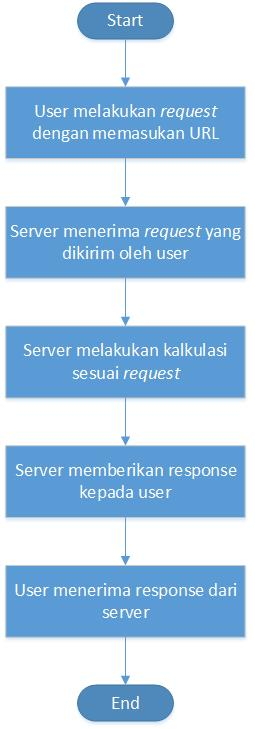
\includegraphics[scale=0.5]{Gambar/flowchartgoogledir.jpg}
				\caption[Flow Chart Alur Layanan Google Direction]{Flow Chart Alur Layanan Google Direction}
				\label{fig:flowchartgoogledir}	
			\end{figure}
			
\section{Analisis permintaan ke layanan Google Direction}
\label{sec:analisisrequestgoogledir}

Sesuai dengan subbab \ref{subsec:permintaanarahgoogledir} permintaan dari google direction ini menggunakan protokol HTTP. Permintaan tersebut menghubungi hostname maps.googleapis.com dengan port default untuk port HTTP yaitu 80. Permintaan tersebut disertai dengan parameter-444`3parameter opsional lainnya untuk mendapatkan data yang diinginkan.

\subsection{Parameter yang digunakan}
\label{subsec:parameterrequestaplikasi}			

Untuk mendapatkan data waktu tempuh yang beragam untuk menganalisis waktu tempuh dari 2 titik sesuai dengan \ref{subsec:parameterpermintaangoogledir}, parameter opsional yang digunakan adalah :  \textbf{departure\_time} dan \textbf{traffic\_model}. Dari memanipulasi kedua parameter tersebut akan menghasilkan data waktu tempuh yang beragam. Selain itu memanipulasi nilai parameter pada \textbf{destination} dan  \textbf{origin} juga akan mempengaruhi data waktu tempuh yang dihasilkan karena pada perhitungan dari masing-masing \textbf{destination} ke \textbf{origin} akan menghasilkan waktu tempuh yang berbeda. Dari masing-masing \textbf{destination} ke \textbf{origin}juga memiliki jam kepadatan tertentu dimana nilai waktu tempuh akan berbeda dengan jam-jam lainnya sesuai dengan \textbf{departure\_time}. Parameter \textbf{traffic\_model} ini juga mempengaruhi nilai yang watu tempuh dikeluarkan tergantung model apakah yang digunakan yang telah dibahas pada subbab \ref{subsubsec:parameteropsional}.

\begin{lstlisting}[caption= Traffic\_model : best\_guess, captionpos=b, label=listing:trafficmodelbestguess]
	https://maps.googleapis.com/maps/api/directions/json?...traffic_model=best_guess
\end{lstlisting}
\begin{lstlisting}[caption= Traffic\_model : optimistic, captionpos=b, label=listing:trafficmodeloptimistic]
	https://maps.googleapis.com/maps/api/directions/json?...traffic_model=optimistic
\end{lstlisting}
\begin{lstlisting}[caption= Traffic\_model : pessimistic, captionpos=b, label=listing:trafficmodelpessimistic]
	https://maps.googleapis.com/maps/api/directions/json?...traffic_model=pessimistic
\end{lstlisting}

pada listing diatas, merupakan contoh dari permintaan yang akan digunakan pada perangkat lunak. Berikut adalah penjelasannya :
\begin{itemize}
	\item pada listing \ref{listing:trafficmodelbestguess} menggunakan traffic model best\_guess, dimana traffic model tersebut berpengaruh pada waktu tempuh yang akan dihitung sesuai dengan perkiraan keadaan nyata.
	\item pada listing \ref{listing:trafficmodeloptimistic} menggunakan traffic model optimistic, dimana traffic model tersebut berpengaruh pada waktu tempuh yang akan dihitung sesuai dengan jika tidak memperhitungkan kemacetan.
	\item pada listing \ref{listing:trafficmodelpessimistic} menggunakan traffic model pessimistic, dimana traffic model tersebut berpengaruh pada waktu tempuh yang akan dihitung sesuai dengan jika memperhitungkan kemacetan.
\end{itemize}

Berikut adalah contoh hasil dari ketiga traffic model sebagai perbandingan. Ketiga contoh permintaan menggunakan parameter alamat asal Universitas Katolik Parahyangan, alamat tujuan Komplek Amaya Residence dan waktu perjalanan pada pukul 12.00 : 

\begin{lstlisting}[caption= Contoh Hasil best\_guess, captionpos=b]
{
   "geocoded_waypoints" :[
		...
	 "routes" : [
	 ...
		 "legs" : [
		 ...
			"duration_in_traffic" : {
          "text" : "43 menit",
          "value" : 2603
	    },
		  ...
	 "status" : "OK"
}
\end{lstlisting}

\begin{lstlisting}[caption= Contoh Hasil optimistic, captionpos=b]
{
   "geocoded_waypoints" :[
		...
	 "routes" : [
	 ...
		 "legs" : [
		 ...
			"duration_in_traffic" : {
          "text" : "35 menit",
          "value" : 2099
	    },
		  ...
	 "status" : "OK"
}
\end{lstlisting}

\begin{lstlisting}[caption= Contoh Hasil pessmistic, captionpos=b]
{
   "geocoded_waypoints" :[
		...
	 "routes" : [
	 ...
		 "legs" : [
		 ...
			"duration_in_traffic" : {
          "text" : "1 jam 3 menit",
          "value" : 3759
	    },
		  ...
	 "status" : "OK"
}
\end{lstlisting}

\section{Analisis response dari layanan Google Directions}
\label{sec:analisisresponsegoogledir}

Pada saat melakukan permintaan, Server akan memberikan \textit{response} dengan format JSON. Response yang diterima adalah hasil perhitungan dari \textit{origin} ke \textit{destination}. Dari response ini terdapat banyak data didalamnya.

Data waktu tempuh pada hasil response permintaan ada pada \textit{duration\_in\_traffic} dimana \textit{duration\_in\_traffic} ini adalah salah satu elemen dari \textit{legs} (subsubbab \ref{subsubsec:elemenlegs}) yang merupakan sebuah \textit{json array} dan \textit{legs} ini sendiri adalah salah satu elemen dari \textit{routes} yang merupakan elemen dari \textit{response} yang diterima.
 
\begin{lstlisting}[caption= Hasil \textit{response} Google Directions, captionpos=b, label=lisiting:contohhasilpermintaan]
{
   "geocoded_waypoints" :[
		...
	 "routes" : [
	 ...
		 "legs" : [
		 ...
			"duration_in_traffic" : {
          "text" : "57 menit",
          "value" : 3439
	    },
		  ...
	 "status" : "OK"
}
\end{lstlisting}

Pada contoh hasil permintaan yang ada pada listing \ref{lisiting:contohhasilpermintaan}, terdapat tag-tag dari format JSON yang didapatkan. Yang akan diekstraksi adalah data \textit{duration\_in\_traffic} dimana tag tersebut merupakan bagian dari legs dan legs merupakan bagian dari routes dari hasil permintaan. Didalam \textit{duration\_in\_traffic} terdapat dua pasang data yaitu pasangan \textit{text} dan pasangan \textit{value}. Pasangan \textit{text} merupakan pasangan data dengan \textit{key}-nya adalah \textit{text} dan \textit{value} yang merupakan string dimana hasil konversi dari dari pasangan \textit{value} dalam satuan menit yang dibulatkan. Pasangan \textit{value} merupakan pasangan data dengan \textit{key}-nya adalah \textit{value} dan \textit{value} yang merupakan bilangan yang merepresentasikan waktu tempuh dalam satuan detik.

\section{Gambaran Umum Perangkat Lunak}
\label{sec:gambaranumum}

Perangkat lunak yang akan dibangun adalah perangkat lunak untuk menghitung waktu tempuh dari 2 titik yang ditentukan. Perangkat lunak yang akan dibangun ini bertujuan untuk membantu menganalisis pada jam berapakah waktu tempuh paling cepat dalam waktu 1 minggu terhitung dari hari senin. Selain itu, perangkat lunak ini bertujuan untuk membantu pengambilan keputusan pengguna untuk menentukan pada jam berapakah pengguna melakukan perjalanan agar tidak terjebak dalam kemacetan. Perangkat lunak ini berjalan pada protokol HTTP. Perangkat lunak ini dibangun pada perangkat komputer(desktop) yang berfungsi sebagai penghitung waktu tempuh dengan memanfaatkan Google Direction API. Perangkat lunak mengeluarkan \textit{output} berupa file yang berekstensi .csv untuk mencatat seluruh data yang diterima oleh perangkat lunak dari layanan Google Direction dan menggunakan aplikasi \textit{Microsoft Excel} untuk membantu menganalisis data dengan cara me-\textit{generate} bagan secara manual oleh pengguna.
Perangkat lunak ini akan diuji coba sesuai dengan sampel sebagai berikut : menghitung  waktu tempuh antar lokasi yang beralamat Jln. Ciumbuleuit No.94 dan Komplek Amaya Residence; menghitung  waktu tempuh antar lokasi yang beralamat Jln. Ciumbuleuit No.94 dan Komplek Taman Puspa Indah. Penetapan sampel untuk memudahkan mendapatkan waktu tempuh dengan alamat yang statis dan memudahkan untuk output yang dikeluarkan.
						
\section{Analisis Perangkat Lunak}
\label{sec:analisispl}

Perangkat lunak yang akan dibangun adalah perangkat lunak yang dapat melakukan penghitungan waktu tempuh tercepat berdasarkan \textit{request-request} yang dikirimkan oleh user dalam jangka waktu 1 minggu terhitung dari senin. perangkat lunak dibangun dengan menggunakan bahasa pemrograman Java dan membutuhkan \textit{library} jsoup yang akan digunakan untuk membantu perancangan dan pengimplementasian perangkat lunak yang akan dibangun oleh penulis. Berikut adalah fitur-fitur yang akan dibangun pada perangkat lunak:

\begin{enumerate}
	\item Mengekstaksi data waktu tempuh dari keluaran \textit{response} Google Direction dan menampilkan pukul berapa yang memiliki waktu tempuh terbaik dalam kurun waktu 1 minggu.
	\item Menyimpan data-data waktu tempuh dari keluaran \textit{response} Google Direction pada file berekstensi .csv.
\end{enumerate}
 
\section{Analisis \textit{Use Case}}
\label{sec:analisisusecase}

\subsection{Diagram \textit{Use Case}}
\label{subsec:diagramusecase}

Diagram use case pada perangkat lunak yang akan dibangun hanya mengandung satu aktor, yaitu User. Diagram use case dapat dilihat pada Gambar \ref{fig:diagramusecase}.

\begin{figure}[H]
				\centering		
				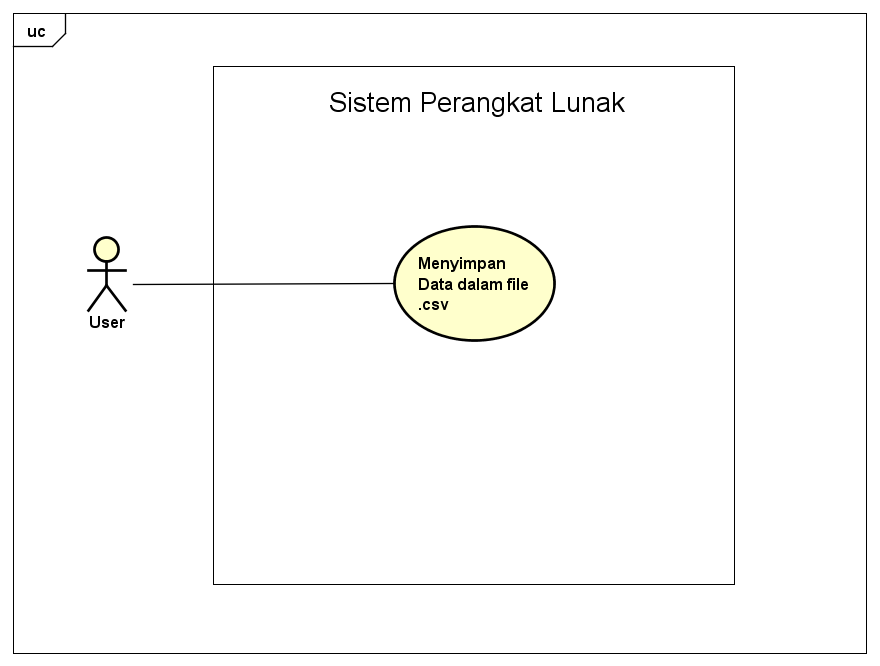
\includegraphics[scale=0.45]{Gambar/UseCaseDiagram.png}
				\caption[Diagram \textit{Use Case} Perangkat Lunak]{Diagram \textit{Use Case} Perangkat Lunak}
				\label{fig:diagramusecase}	
\end{figure}
			
Berdasarkan subbab \ref{sec:analisispl}. dari fitur yang akan dibuat, dibentuk 4 \textit{use case} antara lain:
\begin{itemize}
\item \textbf{Menyimpan Data dalam file .csv}, User dapat menyimpan data dari penghitungan antara sampel dan UNPAR.
\item \textbf{Request JSON}, sistem melakukan request untuk menghitung antara sampel dan UNPAR.
\item \textbf{Ekstraksi data}, sistem mengekstraksi data dari hasil permintaan.
\item \textbf{Menampilkan hasil terbaik dan terburuk}, sistem menampilkan waktu tempuh terbaik dan terburuk dari hasil ekstraksi data.
\end{itemize}

\subsection{Skenario \textit{Use Case}}
\label{subsec:skenariousecase}

\begin{enumerate}
	\item Menghitung Waktu Tempuh
	
	\begin{itemize}
		\item Nama : Menyimpan Data dalam file .csv.
		\item Aktor : User.
		\item Deskripsi : Menyimpan data dari hasil penghitungan dari tempat asal tempat asal ke tempat tujuan.
		\item Kondisi awal : User memulai program. 
		\item Kondisi akhir : User berhasil menyimpan data dan membuka file tersebut dengan bantuan excel. 
		\item Skenario Utama : \\
\begin{table}[H]
\centering
\begin{tabular}{|p{1cm}|p{4cm}|p{4cm}|}
\hline
No & Aksi Aktor   & Reaksi Sistem                             \\ \hline
1                                 & User memulai program                        & Sistem menampilkan GUI dari perangkat lunak                             \\ \hline
2                                 & User melakukan input                        &                                                                         \\ \hline
3                                 & User menekan tombol save                    & Sistem melakukan "`Ekstraksi data"' seusai dengan input dari user                      \\ \hline
4                                 &                                             & Sistem menampilkan layar untuk penyimpanan file                         \\ \hline
5                                 & User melakukan input untuk penyimpanan file & Sistem melakukan penyimpanan file seusai input dari user                \\ \hline
6                                 &                                             & Sistem melakukan "`Menampilkan hasil terbaik dan terburuk"' \\ \hline
7                                 &User menakan tombol                                             & Sistem mebuka file tersebut dengan menggunakan aplikasi Microsoft Excel \\ \hline
\end{tabular}
\end{table}
\item Eksepsi : 
		\begin{itemize}
			\item tidak ada model traffic yang dipilih.
			\item user belum memilih sampel mana yang akan dihitung.
			\item user belum memilih tanggal.
			\item user memilih tanggal pada masa lampau dan hari ini.
		\end{itemize}
		\end{itemize}
	
		\begin{itemize}
		\item Nama : Ekstraksi data.
		\item Aktor : -.
		\item Deskripsi : Mengekstaksi data dari hasil request.
		\item Kondisi awal : Sistem telah melakukan "`Request JSON"'. 
		\item Kondisi akhir : Sistem menghimpun data ekstraksi. 
		\item Skenario Utama : \\
\begin{table}[H]
\centering
\begin{tabular}{|p{1cm}|p{4cm}|p{4cm}|}
\hline
\multicolumn{1}{|c|}{\textbf{No}} & \multicolumn{1}{c|}{\textbf{Aksi Aktor}}    & \multicolumn{1}{c|}{\textbf{Reaksi Sistem}}                             \\ \hline
1                                 &                        & Sistem mengekstraksi JSON dari hasil request                             \\ \hline
2                                 & &Sistem menyimpan hasil ekstraksi kedalam struktur data\\ \hline
\end{tabular}
\end{table}
	\end{itemize}	


	\begin{itemize}
		\item Nama : Manampilkan hasil waktu tebaik dan terburuk.
		\item Aktor : -.
		\item Deskripsi : Menampilkan hasil waktu tempuh terbaik dan waktu tempuh terburuk.
		\item Kondisi awal : Sistem telah mengekstaksi data. 
		\item Kondisi akhir : Sistem menampilkan hasil waktu tempuh terbaik dan terburuk dengan option pane. 
		\item Skenario Utama : \\
\begin{table}[H]
\centering
\begin{tabular}{|p{1cm}|p{4cm}|p{4cm}|}
\hline
\multicolumn{1}{|c|}{\textbf{No}} & \multicolumn{1}{c|}{\textbf{Aksi Aktor}}    & \multicolumn{1}{c|}{\textbf{Reaksi Sistem}}                             \\ \hline
1                                 &                        & Sistem menampilkan hasil waktu terbaik dan terburuk pada option pane                             \\ \hline
\end{tabular}
\end{table}
\end{itemize}	


\begin{itemize}
		\item Nama : Request JSON.
		\item Aktor : -.
		\item Deskripsi : Melakukan permintaan untuk penghitungan waktu tempuh antara alamat awal dan alamat tujuan.
		\item Kondisi awal : Sistem telah menerima input dari user. 
		\item Kondisi akhir : Sistem mendapatkan hasil dari permintaan. 
		\item Skenario Utama : \\
\begin{table}[H]
\centering
\begin{tabular}{|p{1cm}|p{4cm}|p{4cm}|}
\hline
No & Aksi Aktor    & Reaksi Sistem                             \\ \hline
1                                 &                        & Sistem menginisialisasi program sesuai inputan dari user                             \\ \hline
2                                 & &Sistem melakukan request ke server\\ \hline
3                                 & &Sistem mendapatkan hasil balasan dari server\\ \hline
\end{tabular}
\end{table}
\end{itemize}	
\end{enumerate}

\section{Analisis Kelas}
\label{sec:analisisclassdiagram}

Diagram kelas analisis untuk perangkat lunak ditunjukkan pada Gambar \ref{fig:classdiagramawal}

\begin{figure}[H]
				\centering		
				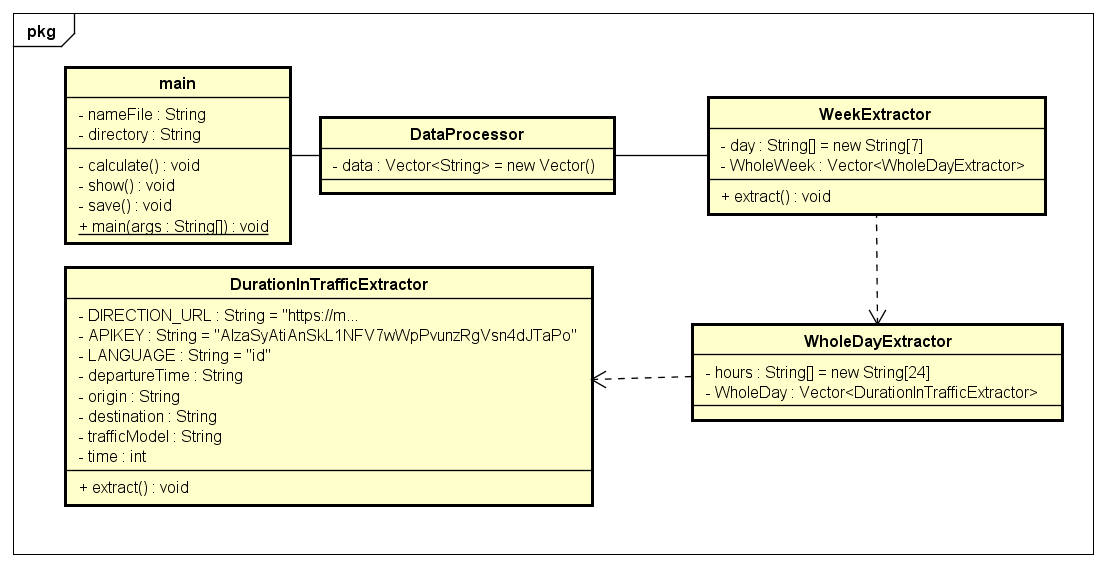
\includegraphics[scale=0.4]{Gambar/ClassDiagram.png}
				\caption[Diagram Kelas untuk Perangkat Lunak]{Diagram Kelas untuk Perangkat Lunak}
				\label{fig:classdiagramawal}	
			\end{figure}
Penjelasan dari kelas-kelas lainnya sebagai berikut:
\begin{enumerate}
	\item \textbf{DurationInTrafficExtractor} adalah kelas yang bertugas untuk mengirimkan permintaan ke layanan Google Direction dan menekstraksi data waktu tempuh.
	\item \textbf{WholeDayExtractor} adalah kelas yang bertugas menekstraksi waktu tempuh dalam 1 hari.
	\item \textbf{WholeWeekExtractor} adalah kelas yang bertugas untuk menekstraksi waktu tempuh dalam 1 minggu.
	\item \textbf{DataProsesor} adalah kelas yang bertugas sebagai tempat penyimpanan data dan bertugas untuk proses penyimpanan data ke dalam file.
	\item \textbf{main} adalah kelas yang bertugas sebagai tampilan utama pada perangkat lunak ini.
\end{enumerate}